\documentclass[conference]{IEEEtran}

\usepackage[pdftex]{graphicx}
\usepackage[]{subfigure}
% correct bad hyphenation here
\hyphenation{op-tical net-works semi-conduc-tor}


\begin{document}
%
% paper title
% can use linebreaks \\ within to get better formatting as desired
\title{Movie Recommendation System based on Self-Organizing Maps}


% author names and affiliations
% use a multiple column layout for up to three different
% affiliations
\author{\IEEEauthorblockN{Kaivan Wadia}
\IEEEauthorblockA{Department of Computer Science\\
The University of Texas at Austin\\
Austin, Texas \\
Email: kwadia@cs.utexas.edu}
\and
\IEEEauthorblockN{Pulkit Gupta}
\IEEEauthorblockA{Department of Computer Science\\
The University of Texas at Austin\\
Austin, Texas \\
Email: pulkit@cs.utexas.edu}}


% make the title area
\maketitle


\begin{abstract}
%\boldmath
A Self-Organizing Map is a neural network technique in the domain of unsupervised learning. A SOM is typically trained to produce a low-dimensional, categorized representation (typically two-dimensional) of a high-dimensional input space. Recommender systems suggest artifacts to a user, for example, suggestions about movies or music a user might like, or items the user might like to purchase. Recommender systems are typically seen as a field closely related to Information Retrieval (IR), and IR methods are most commonly used to implement such systems. This paper presents a novel method to implement a recommender system based on SOMs. Working with a subset of the Internet Movie Database, we show that our system performs considerably better than chance, but worse than the state of the art. We also discuss ways in which our system can be improved and better evaluated.  
\end{abstract}

\IEEEpeerreviewmaketitle



\section{Introduction}
% no \IEEEPARstart
Self-Organizing Maps (SOM) are a class of Neural Network algorithms in the unsupervised-learning category. The central property of a SOM is that it forms a nonlinear projection of a high-dimensional input space on a regular, low-dimensional (usually two-dimensional) grid \cite{kohonen1995springer}. The central idea is that the SOM can discover underlying patterns or structure in the data, and thereby effectively cluster the input data items as well as represent topological relationships between them. The original SOM algorithm was invented by Professor Teuvo Kohonen in 1981-82, and since then a number of different versions of the algorithm, as well as various generalizations and extensions to it, have been developed.

Recommendations are a part of everyday life. In a world where we often have to make consumption choices without having sufficient knowledge of, or experience with, possible alternatives, recommender systems have an important part to play. Typically, we rely on information obtained from other people, either directly or indirectly, to make decisions or settle upon a course of action. For example, we might rely on word-of-mouth opinions or online ratings and reviews while deciding which movie to watch. A recommender system essentially automates this process, helping a user quickly and effectively find what he/she is looking for.

The two most common approaches taken by recommender systems are collaborative filtering and content-based filtering. In collaborative filtering, user similarity is calculated to find other, similar users in the system, and recommendations are based on the items that similar users found relevant . This is the approach taken by Amazon - it looks at your purchases, and recommends other items that were purchased by other users who bought the same item. In content-based filtering, recommendations are generated based on items a user previously found relevant. Music recommendations on Pandora radio and Spotify are generally made using content-based filtering.

In a recommender system, the system suggests certain items (or artifacts) contained in the system, based on defined criteria. Recommender systems are different from typical information retrieval systems in one major way - instead of generating results based on an explicit query entered by the user, recommender systems collect information about the user (either implicitly or explicitly) and generate recommendations based on that information.

SOMs, by virtue of their ability to represent high-dimensional data, have a large number of potential applications. WEBSOM \cite{kaski1998websom} is one of the most popular extensions of the SOM. The WEBSOM method can be used to organize large collections of documents, and various algorithms have been developed to implement information retrieval based on WEBSOM. Our project aims to explore the possibility of applying this technique beyond traditional text information retrieval.

In this paper, we present a new method of building a recommender system, based on the WEBSOM project. Our project can therefore be thought of as lying at the intersection of the fields of Information Retrieval and Neural Networks. Our system is a content-based filtering system – it works with a user's movie-watching history and comes up with a list of movies that the user might like. Our initial dataset was a collection of over 1400 movies taken from the Internet Movie Database (IMDb), and we obtained movie-history data from 28 users to evaluate the performance of our system.

This paper is organized as follows: section 2 briefly talks about background and related work. Section 3 describes our architecture, approach and dataset. Section 4 describes the experiments conducted and results obtained. We discuss the results and present possible future directions our work may take in Section 5, before concluding in Section 6.  

% You must have at least 2 lines in the paragraph with the drop letter
% (should never be an issue)


\section{Related Work}
Recommender systems are a relatively new idea, and their history can be traced to Resnick \& Varian \cite{resnick1997recommender}. Adomavicius \& Tuzhilin \cite{adomavicius2005toward} provide a survey of the field of recommender systems, and tracks the advances that have been made. 

Movie recommendation systems have either been based on collaborative-filtering approaches or content-based filtering approaches. Certain systems also take a hybrid approach, using a combination of both techniques. 

Collaborative-filtering systems predict recommendations solely on the basis of the past ratings provided by the user. Based on these ratings the system computes a function which predicts the ratings of movies rated by other users and not rated by the user. Collaborative-filtering systems have traditionally output a predicted rating for each movie rather than a binary value stating whether the user will like or dislike a movie. Such a system computes ratings of unseen movies based on the ratings of other people who have similar preferences to the user. The similarity of users is computed by various statistical techniques. One such system called \textit{Recommender} \cite{basu1998recommendation} computes for each user a subset of users who have ratings similar to the user. This small group of users are called the recommenders for a specific user. The ratings of these recommenders are then used to evaluate the rating of an unrated movie. The recommended movies are then presented to the user as a rank-ordered list based on the rating of each movie.

Content-based recommender systems are based on the non-rating information of a movie. These systems use information such as the director, cast, plot keywords, user reviews and critic reviews to recommend movie to the user. A content-based recommendation system takes as input the description of each movie the user has liked and formulates a procedure that would take as input a movie description and predict whether a user would like that movie or not. These systems try to extrapolate the preferences of the user based on movie descriptions and do not rely on other people’s ratings as in the social-filtering techniques. For each user a separate recommendation procedure is generated based on the movies he/she likes. Similarity in such systems is computed using Euclidean distance or cosine distance. The description of each movie is stored as a vector and can have feature weighting i.e. certain features such as cast and director might have a higher weightage while computing similarity than other features such as plot keywords. Since content-based systems do not rely on the ratings of movies by users a movie can be suggested right after its release as long as the relevant information about that movie is known. This enables content-based systems to include new movies in their database much faster than collaborative-filtering systems.

The idea of using Self-Organizing Maps for tasks related to the categorization and retrieval of information is not a new one. Extensive work in this area was done as part of the WEBSOM project \cite{kaski1998websom}, in which SOMs of large document collections were created and subsequently used for document retrieval based on user queries. The results achieved by using the WEBSOM method on massive document collections can be examined in \cite{lagus2004mining}.


\section{Approach}
The goal of our project is to develop a system that takes as input a set of movies liked by the user and returns another set of movies that are expected to be liked by the user. We use a content-based approach along with Self-Organizing Maps to build our system. SOMs have proved useful in the classification and organization of data such as large document collections, as discussed in the last section. Our approach is to use a SOM to organize and classify a movie database and use this classification to search for movies to recommend to the user. We approach the movie recommendation problem as one of classification, rather than the more common approach of predicting the rating of a movie. Given the movies a user likes, the system needs to predict whether a given movie will be liked or disliked by the user. 

We decided to use SOMs as they have an inherent property of classifying data based on the underlying features of the data. One of the main advantages of using SOMs is that the search space is significantly reduced, and the comparisons can focus on specific, relevant subsets of the collection, leading to faster search. Another notable advantage is the ability to use the SOM representation of a data collection for visualization, promoting the exploration and discovery of new information.

The system we developed classifies movies onto a SOM based on the genre and plot keywords of the movies. Once the map has been trained, to make recommendations for a given user, we collect movies from the map based on the given user’s movie-watching history. We decided to collect twice as many movies as the system had to output to compare against. This proved to be a sufficiently large number while maintaining the computational efficiency advantage of SOMs. Once the set of movies to compare against was determined, the system computed the similarity between the user’s input movies and the collected movies using various methods such as euclidean distance, cosine angle and dot product. The most similar movies were returned to the user as the predictions.

Our system can be thought of as having two major phases - the training phase, where the dataset is organized using the SOM method, and the recommending phase, where a user’s movie-watching history is used to determine a set of movies to recommend. An overview of these phases is presented here, with details in the next section.

\subsection{The Training Phase}
Step 1 - Preprocess the movie dataset and decide on the input features that will be used for training the SOM. 
\vspace{2mm}
\\\indent Step 2 - Train the SOM based on the selected inputs

\subsection{The Recommending Phase}
Step 1 - The available list of movies liked by any given user is converted to a vector matrix representation and fed to the system as input. 
\vspace{2mm}
\\\indent Step 2 - Assuming the system is required to recommend ‘n’ movies, it collects a set of ‘2n’ movies for comparison from the map, either by finding map units corresponding to individual input movies, or by combining the input movies into a single vector. 
\vspace{2mm}
\\\indent Step 3 - The system then compares each of the collected movies with the input movies, again, either by considering the input movies individually, or by combining the input movies into a single vector. A number of different metrics are used to perform these comparisons. 
\vspace{2mm}
\\\indent Step 4 - Finally, the ‘n’ movies that are closest to the user’s history are returned as recommendations. 


\section{Experiments and Results}
We conducted a number of experiments using different sets of features and similarity measures. Below, we describe in detail the setup used for the experiments, and report on some of the significant results we obtained. 

\subsection{Training and Test Data}

The movie collection we had available for this experiment was a collection of over 1,400 movies from the Internet Movie Database (IMDb). The IMDb maintains a massive collection of movies and factual information about those movies. All of our content features were extracted from IMDb, and therefore our method should be extensible to larger datasets. Each movie has the following information: director, cast, genre, plot keywords, user comments and critic reviews. We use the genre and plot keyword fields of each movie to form a representation of the movie. A single movie is represented as a vector where the genres and plot keywords corresponding to it are marked as 1 in the vector. The vector used to describe each movie has 3,771 dimensions. All the movies were also labelled according to the genres it belonged to. We alphabetically concatenated the different genres associated with each movie to come up with the labels. This was useful in presenting a visual classification of the movies using the SOM.

In order to compute a set of movies to recommend to the user we used the movie descriptions of the movies liked by the user as input. We conducted an online survey to collect data from real users. Each user was asked to mark all the movies from our dataset that he/she had watched and liked. We used 50\% of the data from each user as the training input and the other 50\% was used as a test set to compare and evaluate the output of our system against. The input set was chosen randomly by shuffling the user’s movie list and selecting the first half of the shuffled set as the input.

\subsection{SOM Implementation}

To implement the SOM we used the SOM Toolbox Toolkit for MATLAB \cite{vesanto2000som}. It provides a MATLAB Toolbox for implementing a SOM and use it for classification and search. We used two different map sizes for our experiment: a smaller 16x12 units map and a bigger 20x15 units map. We decided to use the online, sequential method of training the map over the batch learning method, based on the arguments presented in \cite{fort2002advantages}. It is worth mentioning that we also tried using the k-means clustering algorithm \cite{hartigan1979algorithm} and Learning Vector Quantization \cite{kohonen1997learning} in addition to simple SOMs, but we gave up on those methods because the classification results obtained were not good enough. 

Initially, we tried using only the genre field to classify the movies on the SOM. This did not provide a good classification as most of the movies were grouped together in a few units of the map, leaving large areas of the map blank. This was because there were only 27 unique genre combinations and therefore they were grouped in a small number of units. Our aim was to achieve an even distribution of movies across the whole map with discernable boundaries between different classifications of movies. After experimenting with various combinations of features such as genres, directors, cast, user comments and plot keywords, we decided to use a combination of genres and plot keywords. It was not very useful to use the directors feature as there were over 900 unique directors in the set which meant that not many directors were credited for multiple movies, and would not contribute to recommending similar movies based on directors. 

The SOM generated by using genres and plot keywords as inputs gave an even distribution of movies with clearly defined classifications. The maximum number of movies in any single unit was 65 in the small map and 45 in the big map. Figure 1(a) shows the number of movie hits in each unit of the map with a grouping of map units into different colors based on the genre combinations. Figure 1(b) shows the labels assigned to each map unit which is based on the dominant genre combination of the movies classified into that unit. Figure 2(a) and Figure 2(b) display a magnified version of the center portion of the maps displayed in Figure 1. In Figure 2, we can see a clear partition between various movies based on their genre combinations.

The training input is used by the system to find the best matching units on the SOM. There were three techniques we used to find the best matching units: (1) Find the best matching unit for each input movie, (2) Sum up the vectors of each input movie to get a single vector, and find the best matching unit for this input vector, and (3) Sum up the vectors as in the previous approach and clamp the final vector so that none of its fields have values greater than 1. Contrary to our expectation, we achieved better performance with the latter two techniques. Once we had found the best matching units, we collected all the movies from those map units to compare against. We set up our algorithm to collect at least twice as many movies as the system was expected to output, for comparison. If the system could not collect enough movies from the best-matching unit, we gathered movies from the second best matching unit and so on, until it gathered the required number of movies.

\subsection{Computing Similarity}

The collected movies are then compared to the input movies to compute their similarity and return the movies which are the most similar to the user. To compute the similarity between movies we used various metrics: (1) Minimum Euclidean distance, (2) Minimum cosine angle between vectors and (3) Maximum dot product. For each of these metrics we had two cases. In the first case we compared a movie with each of the input movies and in the second case we compared a movie with the combined input, generated as described in the previous subsection. During the comparison stage, the system also checks for movies that are already in the input set and discards those movies so as not to return the same movies as the input.

\begin{center}
\begin{figure*}
\centering
\subfigure[Number of hits for each unit on the map]{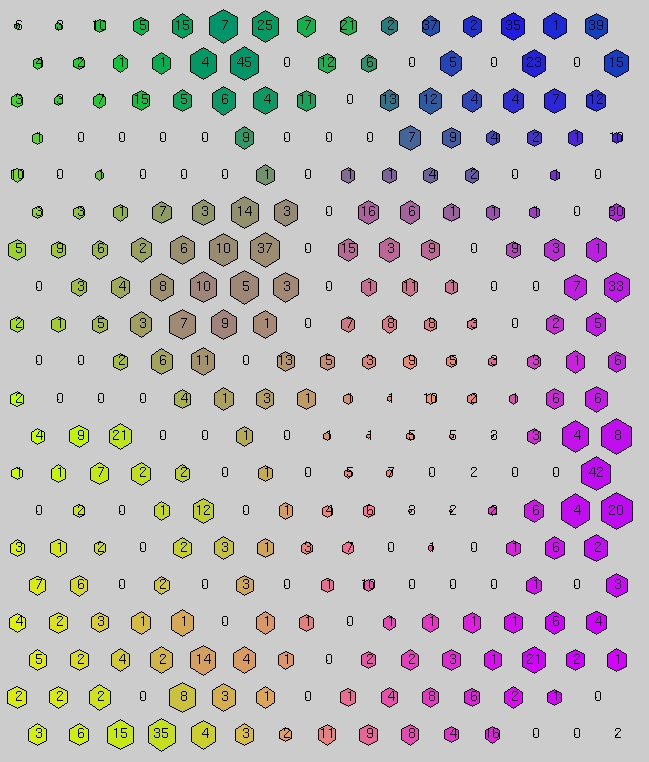
\includegraphics[scale=0.35]{1}}
\subfigure[The label assigned to each map unit]{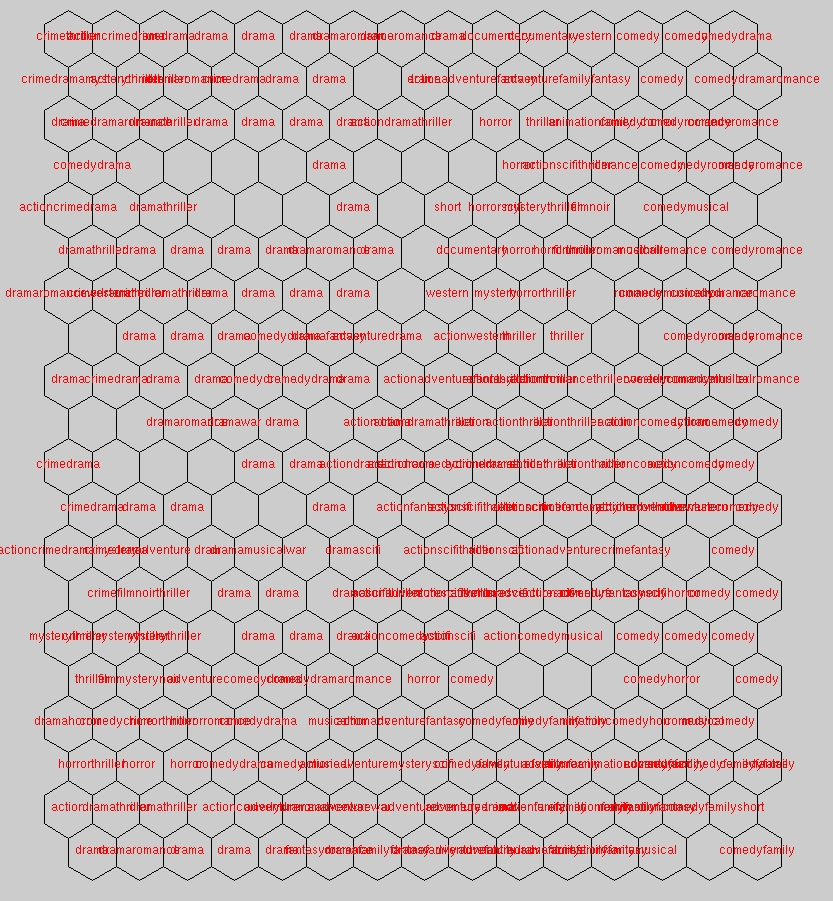
\includegraphics[scale=0.3]{3}}
\caption{Two maps showing the hits per unit and the label of each unit. The label assigned to the unit is the dominant genre combination of the movies in that unit.}
\label{fig1}
\end{figure*}    

\end{center}
\begin{figure*}
\centering
    \subfigure[Number of hits for each unit on the map]{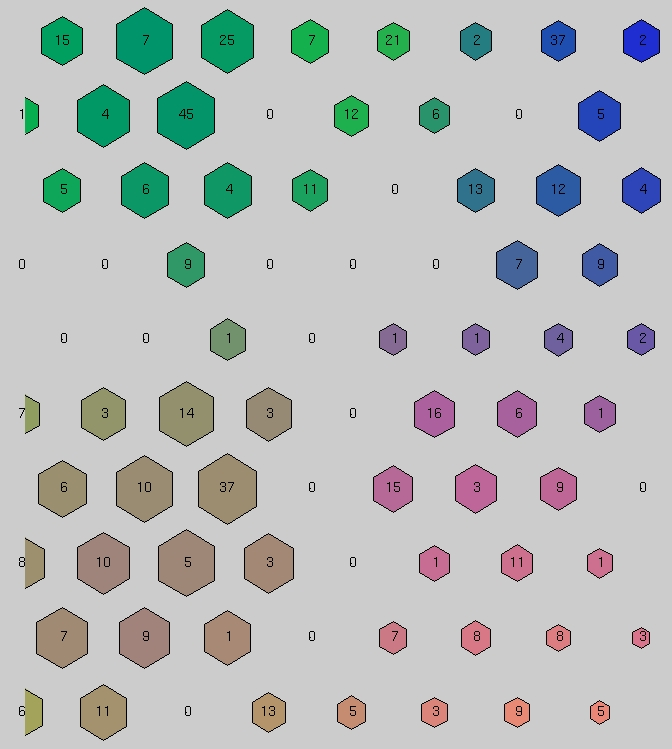
\includegraphics[scale=0.35]{2}}
    \subfigure[The label assigned to each map unit]{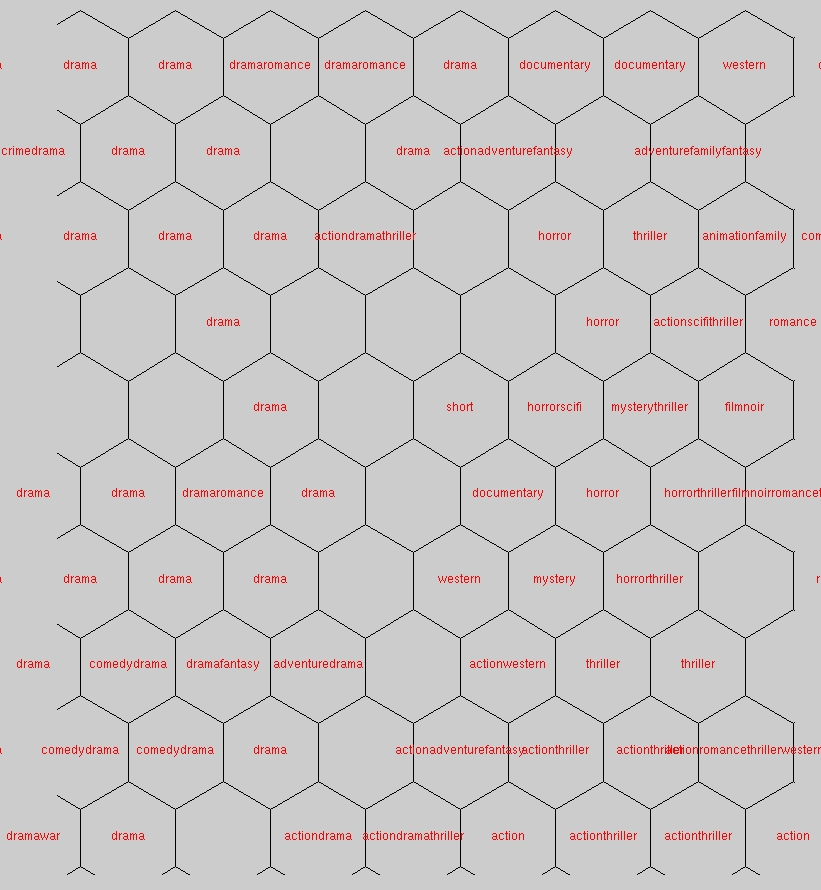
\includegraphics[scale=0.3]{4}}
    \caption{Magnified versions of the center portion of the maps in Fig. \ref{fig1}}
    \label{fig2}
\end{figure*}

\subsection{Evaluation Criteria}

We are interested in predicting whether a movie will be liked or disliked by a user. Many recommendation systems which predict a rating for a given movie evaluate their results on the basis of correlation of ratings. For example they compare their results with actual movie ratings generated by users or critics. This does not work for our recommendation system as the system generates a binary output for each movie which states whether a user will like or dislike a movie. We shall instead use a metric commonly used in information retrieval called \textit{precision}. Precision gives us an estimate of how many movies predicted by our system are actually liked by the user. It is our belief that while recommending movies the user is more interested in a small set of movies that are predicted correctly rather than a large list he/she would have to go through. It is also not suitable to have a very high precision rate as the system should predict a few movies that the user would not usually watch but will hopefully like. After calculating the precision for each user we calculate the average precision by macro-averaging the results for all 28 users.

\subsection{Results}
While training the map we have the ability to set a number of parameters. We used a two phase sequential training process to train the map. The first phase was a general training phase and the second phase was used to fine tune the map. The learning rate was initially set to 0.5 and was gradually reduced to 0.1. For our initial experiment we used the small map with 192 units. The results for the tests on the small map are given in Table 1. The highest macro-average precision we achieved was for the 15.1\% when we used the Euclidean distance measure of similarity and collected the movies based on individual input movies.

For our second experiment we trained a big map of 300 units to classify the movies based on the genres and plot keywords. The other parameters were kept the same as in the training of the small map. The highest macro-averaged precision was again achieved when using the minimum Euclidean distance measure of similarity which was 16.9\%. The movies in this case were collected using the combine and reduce method rather than based on the individual input movies. The Euclidean distance was computed against the combined input vector. When the minimum of the Euclidean distance with each input movie was used, the results were significantly lower. This was also the case when using the dot product similarity measure. We can conclude that it is better to use the combined input vector to compute similarity rather than comparing it with each individual movie. The results of the different prediction methods and collection methods are summarized in Table 2. It can generally be seen that using the combined input vector is better for both prediction and collection. This is because the combined input vector captures more features about the movies the user likes than the individual input vectors by themselves.

\begin{table}[htpb]
\begin{tabular}{c||c|c|c}
Method                          & Individual & Combined & Combined \& Reduced \\
\hline
Euclidean Distance (Individual) & 2.3        & 6.2      & 7.8                  \\
Euclidean Distance (Combined)   & 15.1       & 14.2     & 13.7                 \\
Dot Product (Individual)        & 14.4       & 14.2     & 14.6                 \\
Dot Product (Combined)          & 15.0       & 14.1     & 14.2                 \\
Cosine Similarity (Combined)    & 7.5        & 12.3     & 13.1                
\end{tabular}
\\
\caption{Results of various recommendation approaches using the $16 \times 12$ map}
\end{table}


\begin{table}[htpb]
\begin{tabular}{c||c|c|c}
Method                          & Individual & Combined & Combined \& Reduced \\
\hline
Euclidean Distance (Individual) & 2.2        & 8.3      & 9.8                  \\
Euclidean Distance (Combined)   & 16.0       & 16.2     & 16.9                 \\
Dot Product (Individual)        & 14.7       & 16.2     & 15.8                 \\
Dot Product (Combined)          & 15.7       & 16.4     & 16.8                 \\
Cosine Similarity (Combined)    & 9.3        & 14.4     & 16.1 \\               \end{tabular}
\\
\caption{Results of various recommendation approaches using the $20 \times 15$ map}
\end{table}

\section{Discussion}
In this section, we will analyze the performance of our system, and discuss possible ways in which this performance may be improved.

It is difficult to empirically evaluate the performance of a recommender system. Opinions on movies are subjective and are heavily influenced by individual preferences. As recommender systems have become increasingly popular, a number of metrics for accuracy evaluation of such systems have been proposed and used, as reviewed in \cite{gunawardana2009survey}. The approach we took to evaluation can be seen as incomplete – our evaluation metric may not be truly representative of system performance. Also, while we are working with real user data, in an ideal experiment we would have liked to ask users to watch movies recommended by our system and record their reactions. Since this was not possible, our evaluation metric may potentially have a high degree of error – it is possible that our system is actually generating reasonable recommendations based on the data available to it, but because of the absence of a way to evaluate these recommendations, they are disregarded as errors.

As can be seen, the results produced by our system are significantly better than chance, which suggests that our system is working, at least to some extent. It is, however, not possible to empirically compare the performance of our system against other similar systems because of a number of reasons, the most notable ones being the use of different datasets, and the use of different evaluation metrics. 

As our results indicate, we obtained consistently low percentages for Mean Average Precision (MAP). Keeping in mind the challenges in accurate measurement of system performance, and based on a non-scientific examination of the recommendations returned, we believe that the significantly low performance numbers may not be representative of actual system performance. But we also acknowledge that these numbers may point to shortcomings in the current implementation of our system. We have analyzed and recorded the shortcomings we could identify, and various ways of addressing them, in the following paragraphs. The five main shortcomings we have identified are high input dimensionality, limited context in inputs, feature weighting, lack of a graded rating scale, and small dataset size.

First, the dimensionality of our input space was very high. By using a combination of the genres and plot keywords as inputs to the SOM, we ended up with 3,771 unique inputs, and as a result, a 3,771-dimensional vector space. Because of this, the vector representations of the movies in our set may not have been similar enough to each other in meaningful ways, contributing to the low MAP numbers. The problem of high dimensionality can be solved by dimensionality reduction techniques such as the random-mapping, where the high-dimensional input space is mapped to a lower dimensional space, while maintaining the semantic context of each vector.

Second, because we already had a high-dimensional input space, we were precluded from including additional information that was already available in our dataset as part of the input to our SOM. For example, it may have been possible to include user or critic reviews to achieve better organization, and also incorporate some sense of sentiment in the clustering.

Third, we could have used a more complex processing paradigm, such as the feature weighting in content-based filtering recommender systems, as proposed in \cite{debnath2008feature}. Feature weighting, in conjunction with dimensionality reduction and incorporating additional information from the dataset, would have allowed us to handpick or assign more weight to more relevant features, thereby allowing an unsupervised learning task to benefit from human intuition. This would also have made our system more generalizable – we could have included all features available in the data set, and used different combinations of weights for the features to obtain and compare different organizations of the data.

For ease of data collection, we collected a binary judgment from our test users – we only knew whether they liked a movie or not, whereas actual IMDb data has per-user and average ratings on a 10 point scale. While we had access to the average rating of each film in our dataset, we couldn't use it because of its incompatibility with test data. If we had graded per-user ratings available, we could have modified our algorithm to generate predicted ratings for movies, and used those for coming up with the recommendations, potentially increasing accuracy.

Finally, our SOM couldn't use director or cast information to discriminate between movies in any meaningful way. This was because our dataset was limited in size, and as a result most directors and cast members were credited in only one or a very few movies. If we had a larger dataset, more representative of real-world IMDb data, we could potentially have achieved better organization on the basis of these factors, leading to better recommendations.

Our system has been implemented and tested in a modular way. As a result, the shortcomings we have identified can be corrected in the future, and we expect the performance of our system to improve significantly as a result.

\section{Future Work}
In addition to the system improvements described in the Discussion section, we see a number of directions our work can potentially take in the future. These have been described these in the following paragraphs.

It is possible to modify our algorithm to use an approach that lies between collaborative filtering and content-based filtering. There are multiple ways to do this. One way would be to include user-specific data such as information about movies liked by a user's friends, and information from reviews written by the user and their similarity to other reviews, as inputs to the SOM. This would, however, result in a per-user instance of the movie SOM, which will need to be regenerated periodically. The obvious downsides are constraints on memory and computation power.

This idea can be taken forward in a computationally efficient manner by using a single SOM for the dataset, as happens currently, and based on user-specific information, perform some further computation and enrichment on the recommendations returned by the system. The content-based filtering SOM part of the system can be set up to return a large number of potential movie recommendations, and the collaborative filtering part of the system, based on user-specific information, can be used to refine the results before they are returned to the user.

Also, one of the greatest strengths of Self-Organizing Maps is the ease with which SOM organized data can be visually represented and understood. SOM representations of large data sets can be used to explore unknown parts of the information, or to discover new information without a verbalized query or information need. An important extension of our system can be a GUI to visualize the SOM. This would allow users to explore the map interactively and discover new movies that may be of interest to them.



\section{Conclusion}
In this paper, we have presented a novel implementation of a movie recommendation system based on Self-Organizing Maps. The main advantages of our method are a visual organization of the data based on the underlying structure, and a significant reduction in the size of the search space per result output. Our method was evaluated against real user data collected through an online survey, by using a subset of the movies liked by each user as input to the system. The current results are notably better than random, but significantly worse than the state of the art. However, we feel that with a better dataset and a number of improvements to our method, we may achieve better results. Also, the true worth of our method as a recommender system can only be determined by conducting further experiments with larger datasets.  


\begin{thebibliography}{1}

\bibitem{kohonen1995springer}
Kohonen, Teuvo, and Self-Organizing Maps. ``Springer series in information sciences." Self-organizing maps 30 (1995).

\bibitem{kaski1998websom}
Kaski, Samuel, et al. ``WEBSOM–self-organizing maps of document collections." Neurocomputing 21.1 (1998): 101-117.

\bibitem{resnick1997recommender}
Resnick, Paul, and Hal R. Varian. ``Recommender systems." Communications of the ACM 40.3 (1997): 56-58.

\bibitem{adomavicius2005toward}
Adomavicius, Gediminas, and Alexander Tuzhilin. ``Toward the next generation of recommender systems: A survey of the state-of-the-art and possible extensions." Knowledge and Data Engineering, IEEE Transactions on 17.6 (2005): 734-749.

\bibitem{basu1998recommendation}
Basu, Chumki, Haym Hirsh, and William Cohen. ``Recommendation as classification: Using social and content-based information in recommendation."AAAI/IAAI. 1998.

\bibitem{lagus2004mining}
Lagus, Krista, Samuel Kaski, and Teuvo Kohonen. ``Mining massive document collections by the WEBSOM method." Information Sciences 163.1 (2004): 135-156.

\bibitem{vesanto2000som}
Himberg, Johan, Esa Alhoniemi, and Juha Parhankangas. SOM toolbox for Matlab 5. Helsinki: Helsinki University of Technology, 2000.

\bibitem{fort2002advantages}
Fort, Jean-Claude, Patrick Letremy, and Marie Cottrell. ``Advantages and drawbacks of the Batch Kohonen algorithm." ESANN. Vol. 2. 2002.

\bibitem{hartigan1979algorithm}
Hartigan, John A., and Manchek A. Wong. ``Algorithm AS 136: A k-means clustering algorithm." Applied statistics (1979): 100-108.

\bibitem{kohonen1997learning}
Kohonen, Teuvo. ``Learning vector quantization." Self-Organizing Maps. Springer Berlin Heidelberg, 1997. 203-217.

\bibitem{gunawardana2009survey}
Gunawardana, Asela, and Guy Shani. ``A survey of accuracy evaluation metrics of recommendation tasks." The Journal of Machine Learning Research 10 (2009): 2935-2962.

\bibitem{debnath2008feature}
Debnath, Souvik, Niloy Ganguly, and Pabitra Mitra. ``Feature weighting in content based recommendation system using social network analysis."Proceedings of the 17th international conference on World Wide Web. ACM, 2008.
\end{thebibliography}




% that's all folks
\end{document}


